%% storify source -- a short private paper in the Springer Nature article template.
%% Edit THIS file. Run `python3 build_story.py` to write story.tex, then
%% `latexmk -pdf story.tex`. Never edit story.tex by hand: the build overwrites it.
%%
%% numbers   every number in the prose is a macro the build defines in the data
%%           slot below, or a design constant marked \lit{...}.
%% typed     list every \lit{} constant here: (none yet)
\documentclass[pdflatex,sn-mathphys-num]{sn-jnl}

% crux-sources: __SOURCES__

\usepackage{graphicx}
\usepackage{amsmath}
\usepackage{booktabs}
\usepackage{xcolor}
\usepackage{tikz}
\usetikzlibrary{positioning,arrows.meta,calc}
\usepackage{pgfplots}
\pgfplotsset{compat=1.18}
\usepackage{pgfplotstable}

% A design constant typed in prose, e.g. \lit{95}. It renders its argument unchanged.
\newcommand{\lit}[1]{#1}

% One colour per arm, defined once and reused in every figure.
\definecolor{armA}{HTML}{3F7D7A}
\definecolor{armB}{HTML}{B5462E}

% The build replaces the next line with one \newcommand per number and one
% \pgfplotstableread per chart table.
% __DATA__

\raggedbottom

\begin{document}

\title[Short title]{The answer, stated as a headline}

\author{\fnm{Given} \sur{Family}}
\affil{\orgname{Private draft, \today}}

% Three or four sentences: the question, the design, the answer with its main number
% and its uncertainty, and the main limitation.
\abstract{State the question, how it was tested, the answer, and its main limitation.}

\keywords{keyword, keyword, keyword}

\maketitle

\section{Motivation and background}\label{sec:motivation}
% Why this question matters, what is known, and what was missing. Cite only sources the
% project holds. End on the question in one sentence.

\section{Methods}\label{sec:methods}
% The design as a schematic (Fig.~\ref{fig:design}), the arms with plain names, the
% outcome measure with any mandatory decomposition, the significance criterion, and what
% was fixed before any run (pre-registered). Design constants only, each in \lit{}.

\begin{figure}[t]
\centering
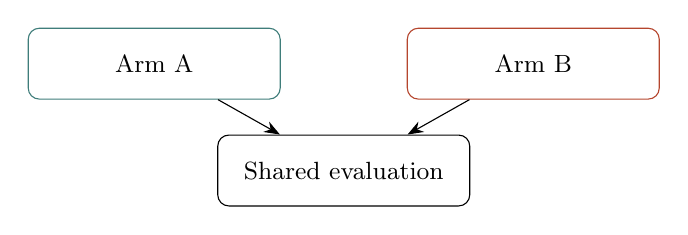
\begin{tikzpicture}[box/.style={draw, rounded corners, align=center,
    minimum width=3.2cm, minimum height=0.9cm, font=\small},
    >={Stealth[length=2mm]}]
  \node[box, draw=armA] (a) {Arm A};
  \node[box, draw=armB, right=1.6cm of a] (b) {Arm B};
  \node[box, below=0.9cm of $(a)!0.5!(b)$] (s) {Shared evaluation};
  \draw[->] (a) -- (s);
  \draw[->] (b) -- (s);
\end{tikzpicture}
\caption{Study design. Name every arm by what it is, never by a code.}\label{fig:design}
\end{figure}

\section{Results and discussion}\label{sec:results}
% One paragraph per claim: quantify, then interpret, then caveat. Every compared value
% carries its 95% confidence interval or its standard deviation across seeds, and a
% difference that fails the significance criterion is labelled by what it fails.
% Keep the negative results.

\begin{figure}[t]
\centering
\begin{tikzpicture}
\begin{axis}[width=0.8\linewidth, height=4.5cm,
    xlabel={Difference (points)}, ytick=data,
    yticklabels from table={\tblExample}{label},
    extra x ticks={0}, extra x tick labels={},
    extra x tick style={grid=major, grid style={gray}}]
  \addplot[only marks, mark=*, color=armA,
      error bars/.cd, x dir=both, x explicit]
    table[x=d, y=y, x error plus=ep, x error minus=em]{\tblExample};
\end{axis}
\end{tikzpicture}
\caption{(a) Say what the chart shows and how to read the error bars.}\label{fig:results}
\end{figure}

\section{Conclusion}\label{sec:conclusion}
% The answer in two or three sentences, the limitations, then the next-step options,
% each with its cost and what it would teach. No ranking and no recommendation.

\backmatter
% Optional: \bibliography{references} with a references.bib beside this file, holding
% only sources the project already has.

\end{document}
